%------------------------------------------------
\section{Eléments technique }


\subsection{Moteur de réécriture}
    \begin{frame}{Un peu D'Histoire}
    \begin{itemize}
          \item Aristid Lindenmayer .
          \item Dans les années 1960. 
    \end{itemize}
   
\end{frame}
\begin{frame}{Grammaire formelle}
\begin{itemize}
    \item Un alphabet V ;  V=\{A,B\}.
    \item Ensemble de constants S ; S=\{-,+,[,]..\}. 
     
    \item Un axiome de départ w ; w=\{A\} .
    \item Ensemble de régles P ; P=\{A:AB,B:A\}.\\
    Notation : G=\{V,S,w,P\}
\end{itemize}   
\end{frame}
\begin{frame}{Exemple avec des Constantes}
     \vspace{1cm}
    \begin{center}
        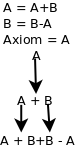
\includegraphics[scale=0.4]{./images/reecriture.png}
    \end{center}
\end{frame}
\begin{frame}{Exemple détaillée}
        \begin{align*}
    \textbf{Alphabet:} & \quad A, B\\
    \textbf{Axiome:} & \quad A \\
    \textbf{Règles:} & \quad A \rightarrow AB \\
    \textbf{Règles:} & \quad B \rightarrow A \\
    \textbf{Constantes:} & \quad Vide \\
    \textbf{Itérations:} & \quad 6
    \end{align*}
 
	   
\end{frame}

\begin{frame}{Exemple détaillée}
    \begin{enumerate}
	       \item[*] n = 0, A
        \item[*] n = 1, AB
     \item[*] n = 2, AB A
     \item[*] n = 3, AB A AB
    \item[*] n = 4, AB A AB AB A
     \item[*]n = 5, AB A AB AB A AB A AB
     \item[*]n = 6, AB A AB AB A AB A AB AB A AB AB A
	   \end{enumerate} 
\end{frame}

\begin{frame}{Génération des L-systèmes standard }
       \begin{itemize}
        
           \item  Une Classe Lsystem .
           \item Une fonction simulation().
           \item Une fonction rotation 2D.
           \item  Une fonction ClaculCoordinate().
           \item Dessiner les points avec drawLine().
       \end{itemize}.
  
\end{frame}

\begin{frame}{}
    \begin{center}
        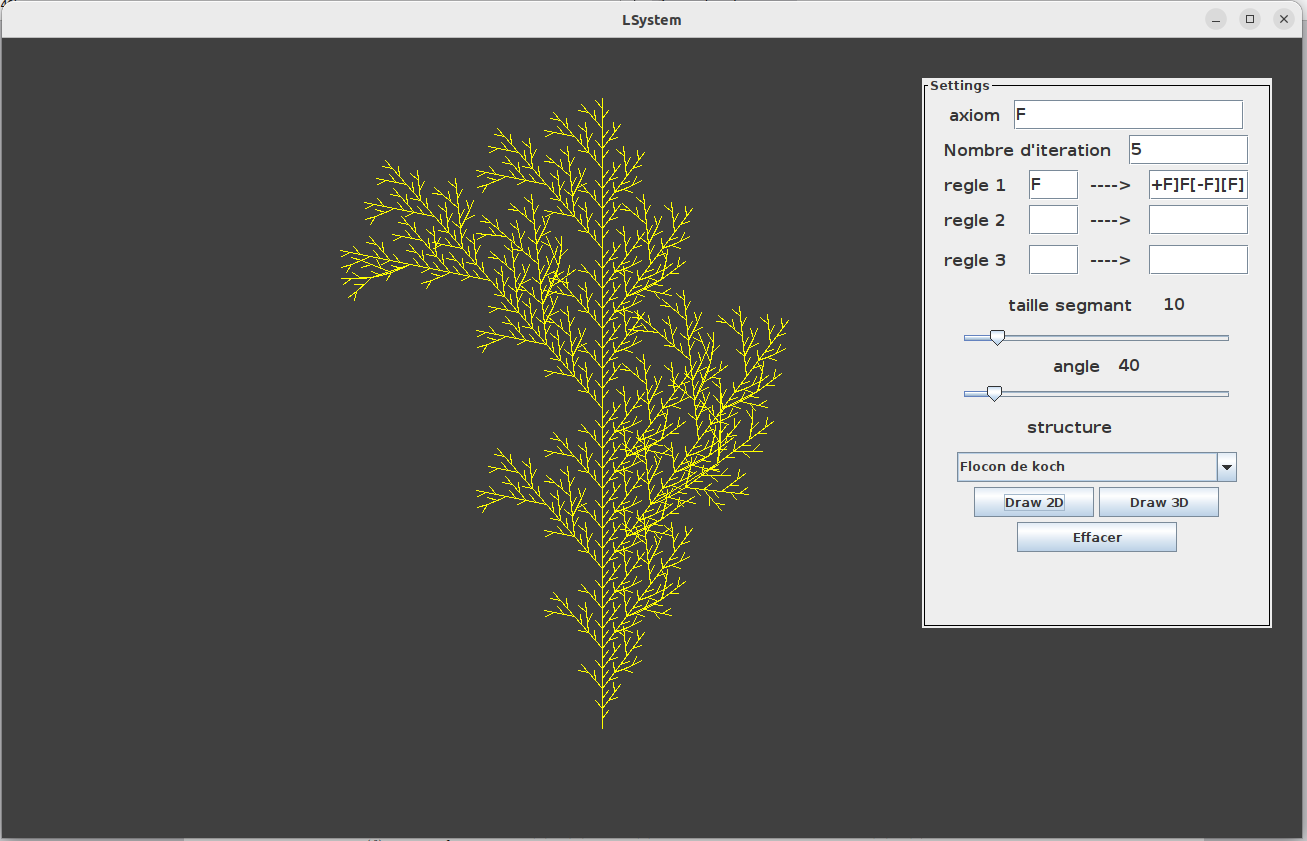
\includegraphics[scale=0.3]{./images/capture3.png}
    \end{center}
\end{frame}
%------------------------------------------------------

    

     
%-----------------------------------------------------------------------



\subsection{Générateur du rendu 2d}
    \begin{frame}{Intérface réalisé}
     \begin{figure}[h!]
      \centering
      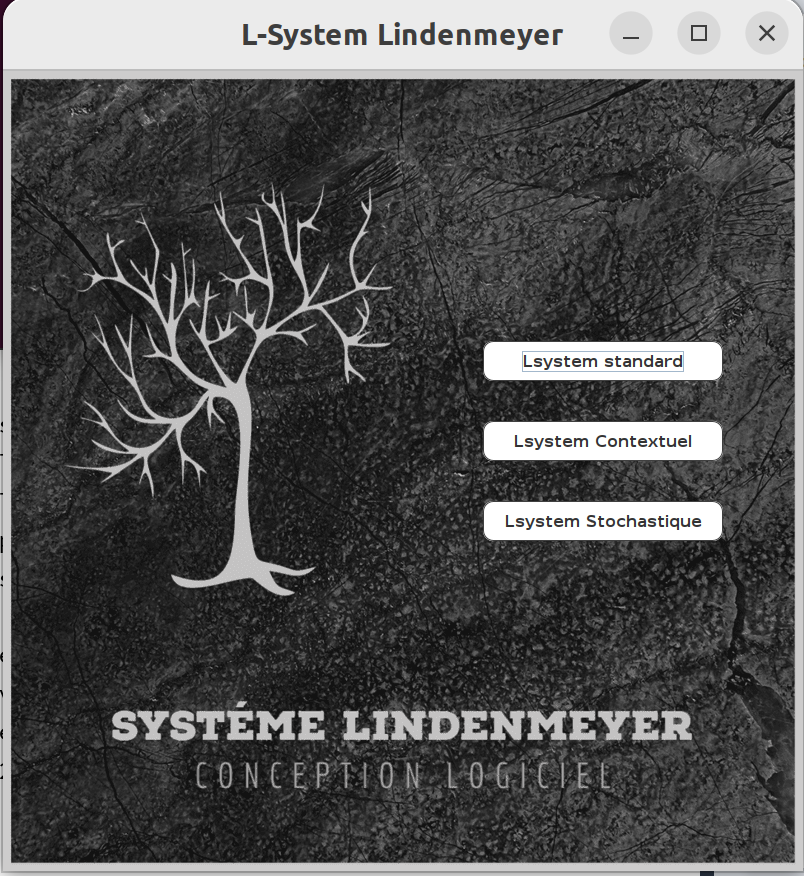
\includegraphics[width=0.5\textwidth]{images/rendu3D.png}
      \caption{Accueil}
      \label{fig:3D}
    \end{figure}
\end{frame}
\begin{frame}{Rendu 2d}
    \begin{itemize}
        \item Le moteur de rendu graphique 2d se base sur une rotation sur les axes X et Y selon l'opérateur de rotation. 
        \vspace{0.2cm}
        \item Nous pouvons voir à travers ce schéma la génération du rendu 2d. 
    \end{itemize}
    \vspace{1cm}
    \begin{center}
        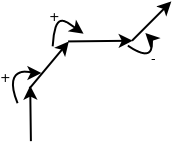
\includegraphics[scale=0.5]{./images/schema.png}
    \end{center}
\end{frame}

\begin{frame}{Rendu 2D}
    \begin{figure}[h!]
      \centering
      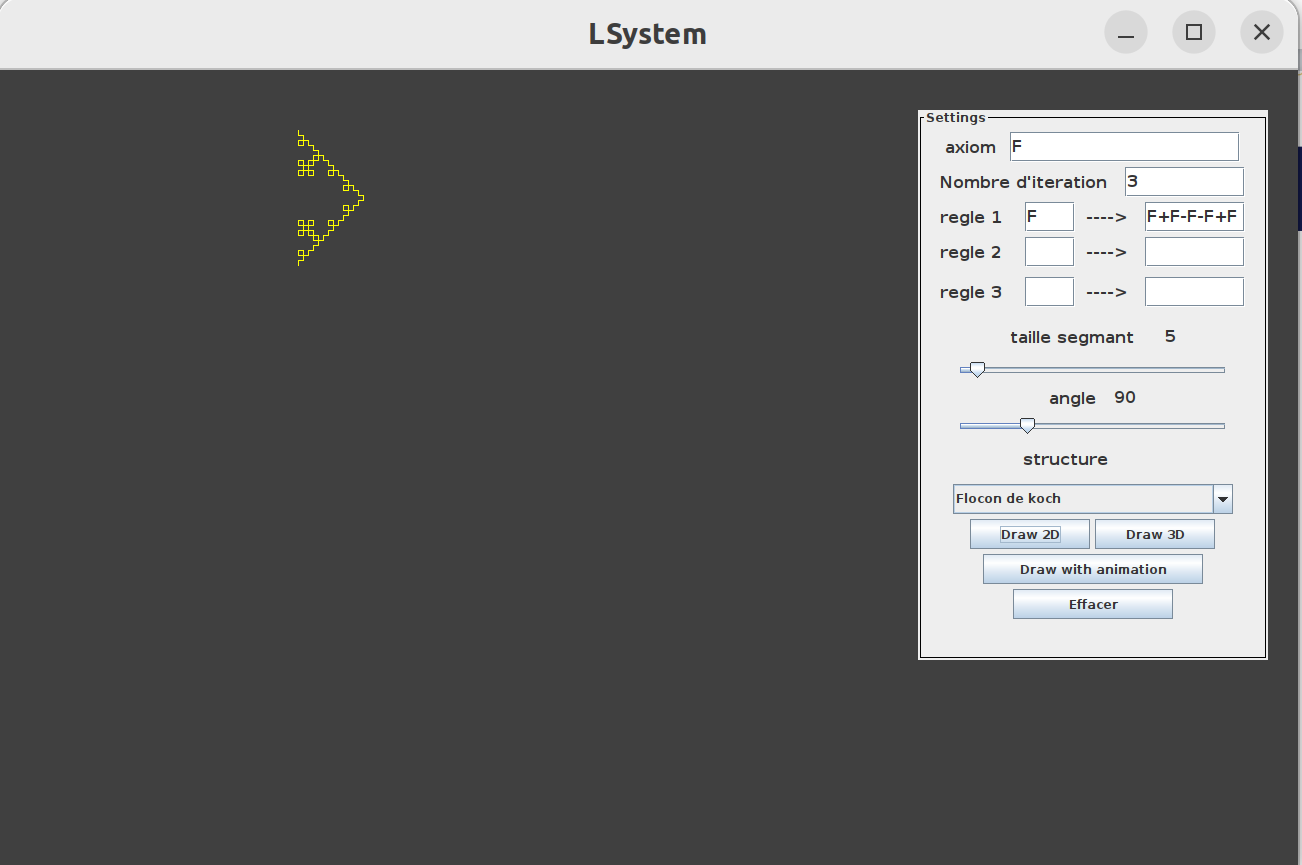
\includegraphics[width=0.5\textwidth]{images/2DD.png}
      \caption{Rendu 2D}
      \label{fig:3D}
    \end{figure}
\end{frame}
\begin{frame}{Rendu 2D}

     \begin{figure}[h!]
      \centering
      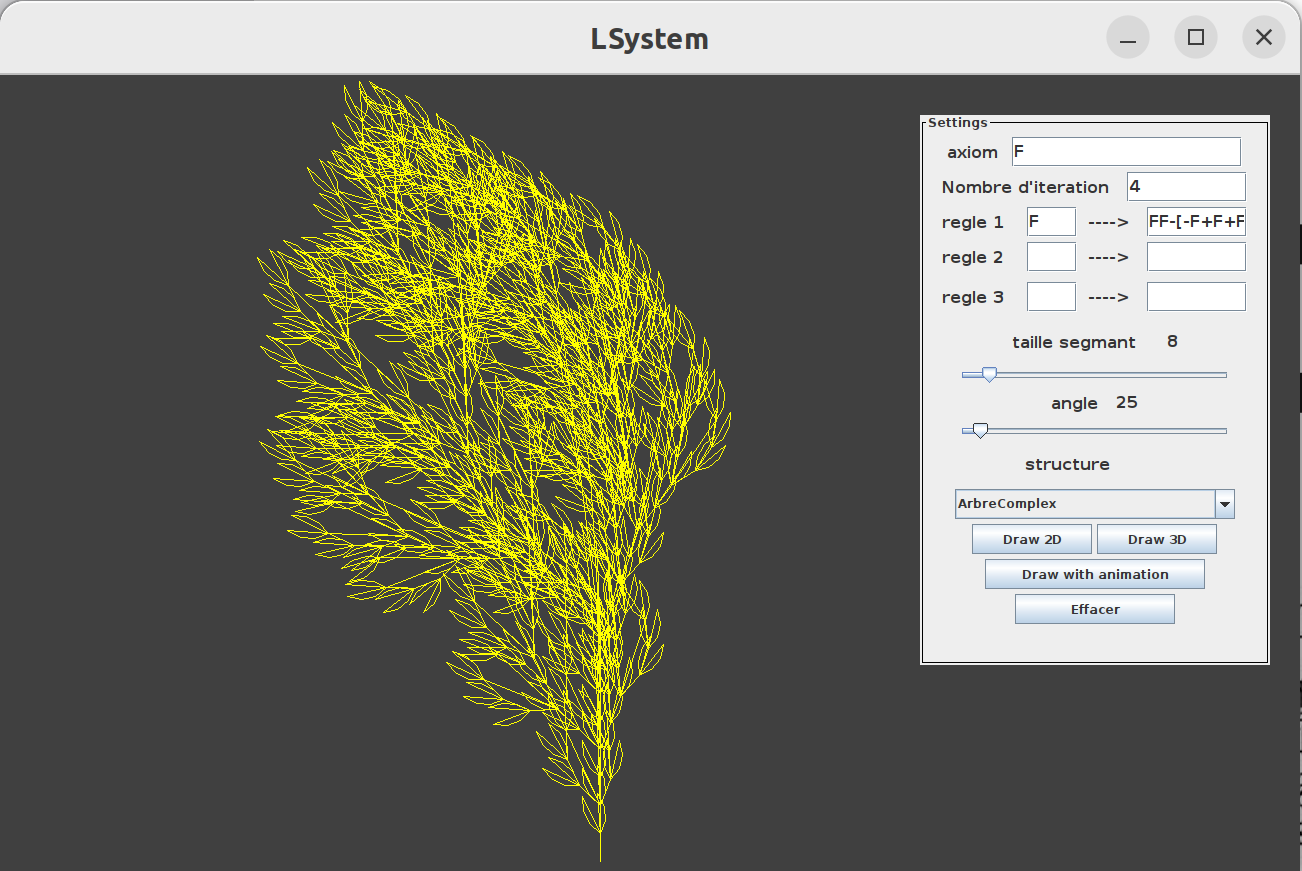
\includegraphics[width=0.5\textwidth]{images/rendu2D.png}
      \caption{Rendu 2D}
      \label{fig:3D}
    \end{figure}

     
\end{frame}
\subsection{Générateur du rendu 3d}

\begin{frame}{Rendu 3d}
    \begin{itemize}
        \item  Le moteur de rendu graphique 3D se base sur une représentation en trois dimensions des structures générées par les L-systèmes, avec une rotation sur les axes X, Y et Z selon les opérateurs de rotation.
    \end{itemize}
\end{frame}
\begin{frame}{Rendu 3d}
    \begin{center}
        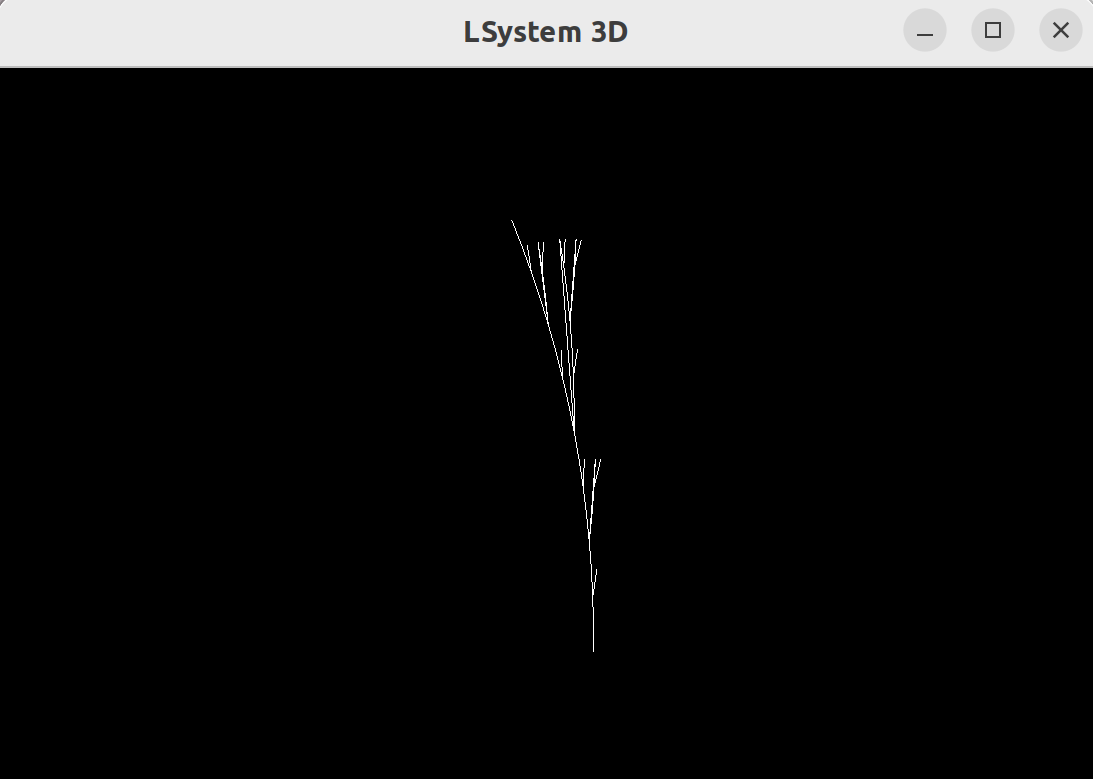
\includegraphics[scale=0.3]{./images/rv.png}
    \end{center}
\end{frame}

\begin{frame}{Rendu 3D}
    \begin{figure}[h!]
      \centering
      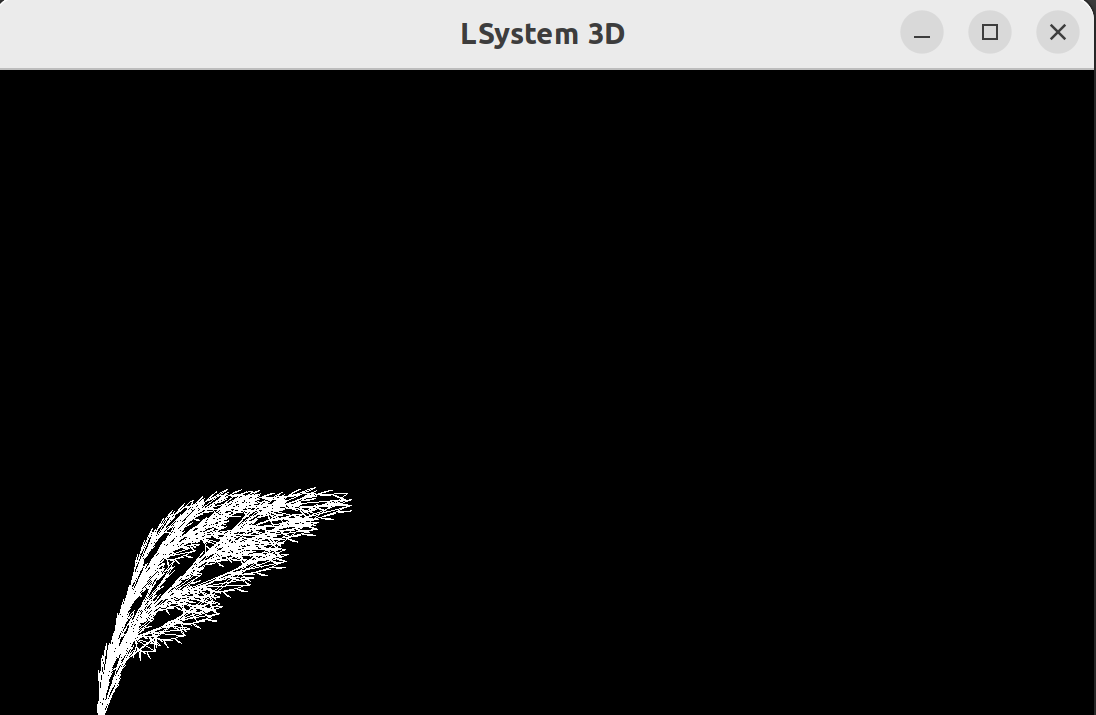
\includegraphics[width=0.5\textwidth]{images/rendu3d.png}
      \caption{Rendu 3D}
      \label{fig:3D}
    \end{figure}


\end{frame}

%--------------------------------------------

  \begin{frame}{Génération des L-systèmes contextuels}
      \begin{itemize}
             \item Les L-systèmes contextuels sont des L-systèmes où les règles de développement des symboles dépendent du contexte. Cela permet de générer des formes plus complexes et réalistes, mais nécessite des règles de développement plus complexes.
         \end{itemize}
    \end{frame}


     \begin{frame}{Génération des L-systèmes contextuels}
        \begin{center}
        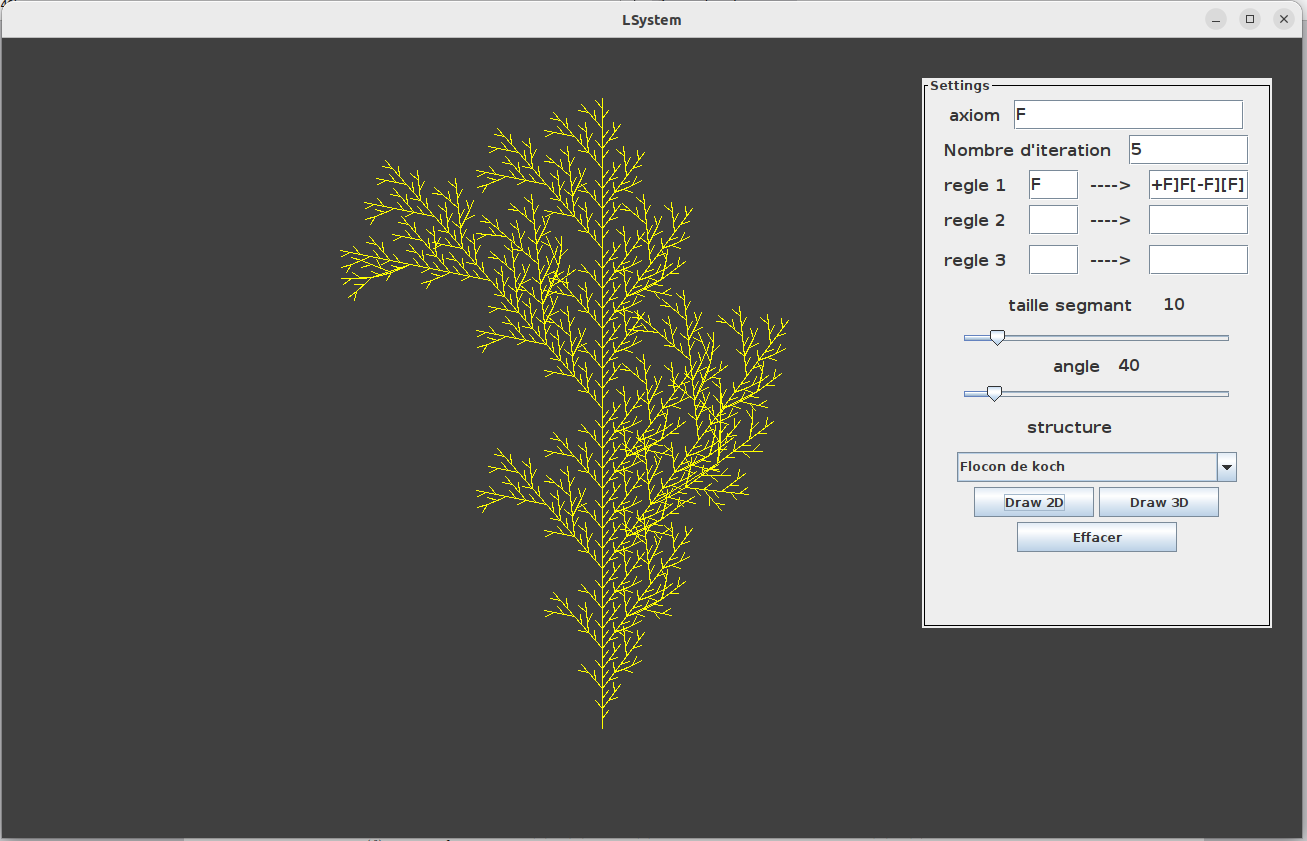
\includegraphics[scale=0.2]{./images/capture3.png}
        
    \end{center}
    \end{frame} 
    
    \begin{frame}{Génération des L-systèmes stochastiques}
         \begin{itemize}
             \item Les L-systèmes stochastiques utilisent des probabilités pour déterminer les règles de développement des symboles, permettant ainsi de produire une variété de formes à partir d'un même L-système de base.
         \end{itemize}
         
    \end{frame}
    
    \begin{frame}{Génération des L-systèmes stochastiques}
        \begin{center}
        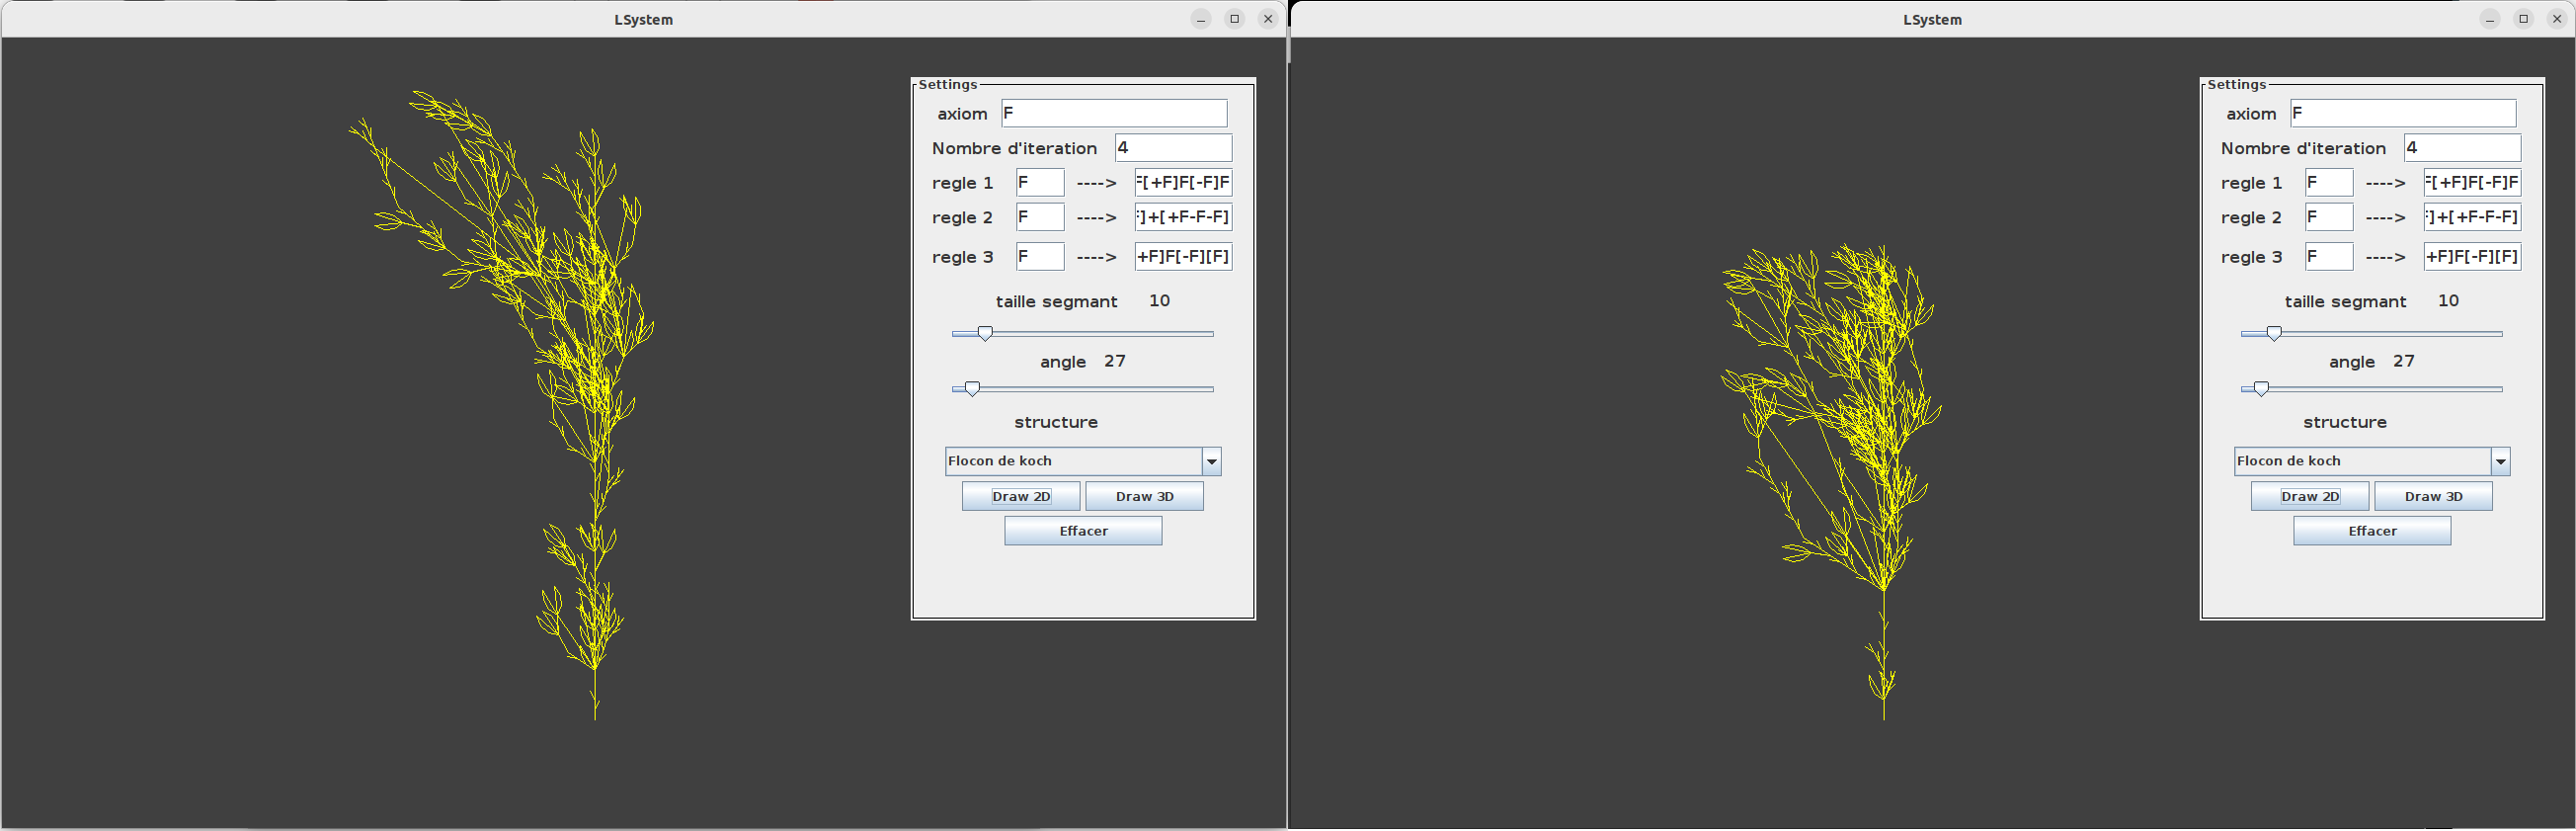
\includegraphics[scale=0.15]{./images/capture1.png}
        
    \end{center}
    \end{frame}
    
  

\begin{frame}{Interface utilisateur + Gestion des erreurs }
    \begin{figure}[h!]
      \centering
      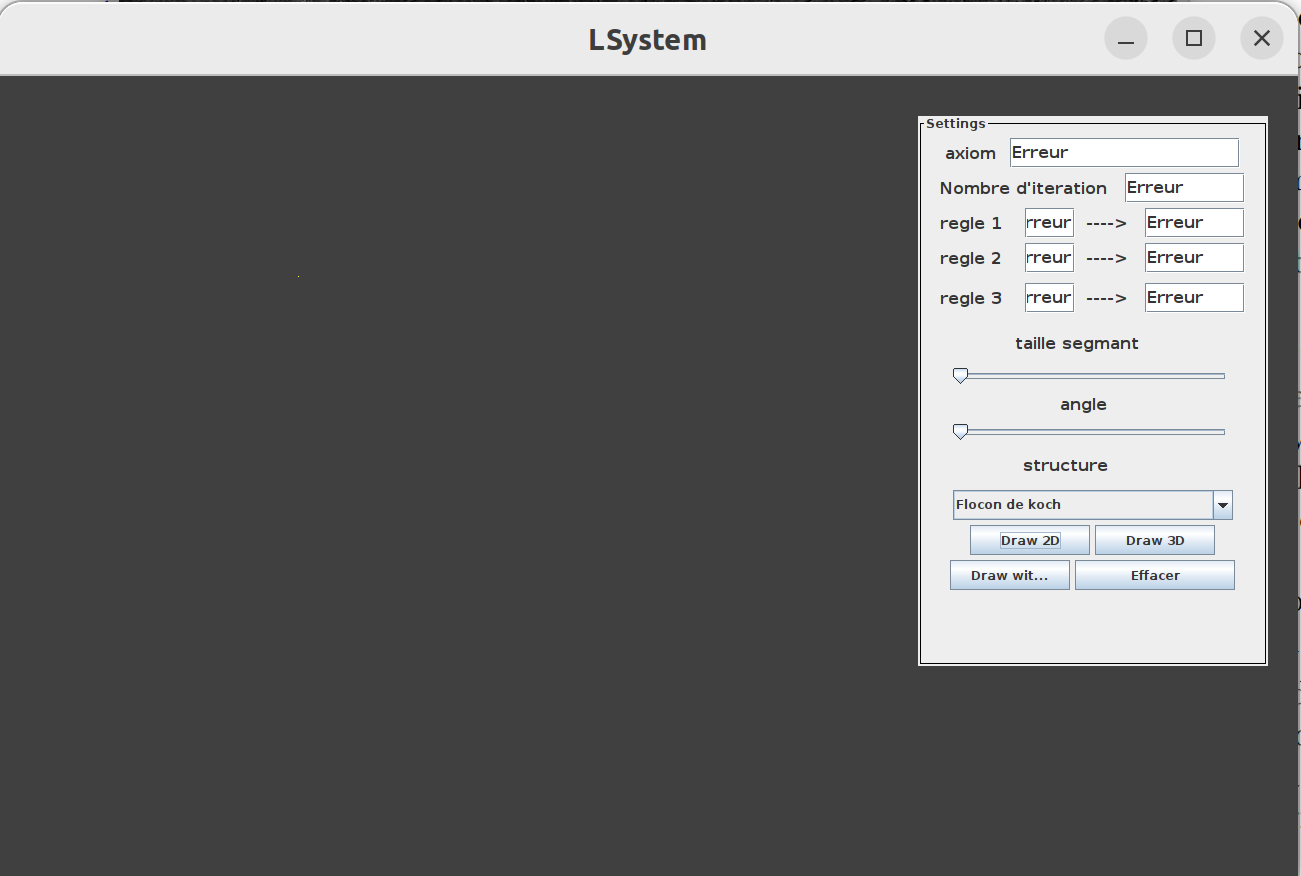
\includegraphics[width=0.5\textwidth]{images/tryandcatch.png}
      \caption{Gérer les exceptions}
      \label{fig:3D}
    \end{figure}
    \end{frame}


\subsection{Fonctionnalitées}
 \begin{frame}{Animation de L-systèmes}
 
        \begin{itemize}
            \item  Visualiser comment les L-systèmes évoluent à mesure qu'ils se développent .

            \item Voir comment les motifs se répètent à différentes échelles

        \end{itemize}
        
\end{frame}
    
\begin{frame}{Timer}
        \begin{figure}[h!]
      \centering
      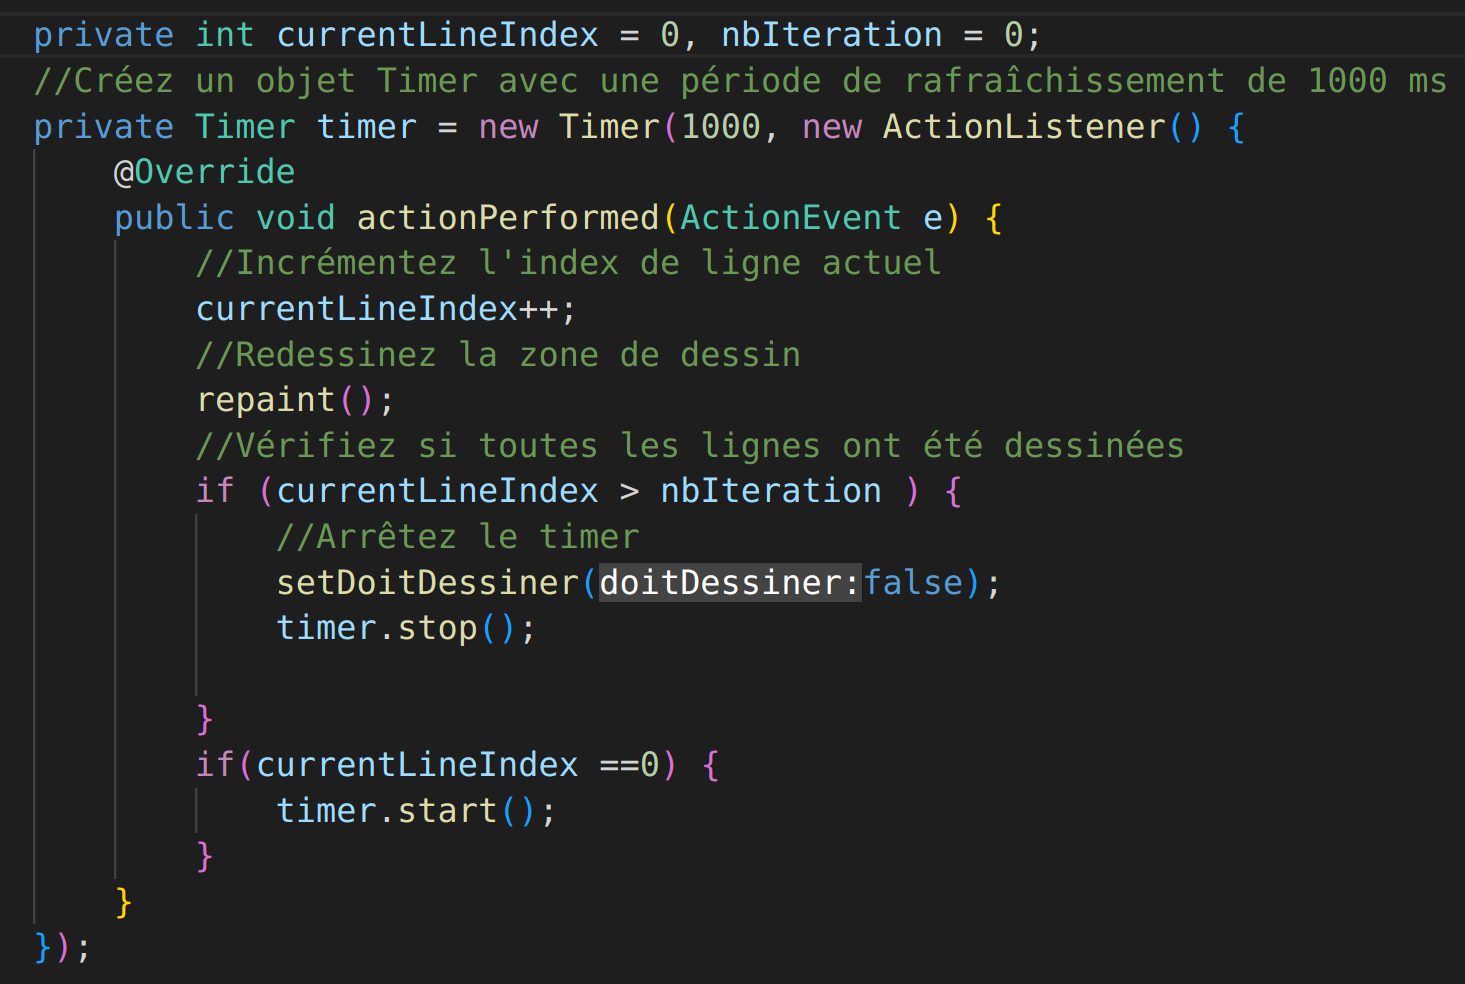
\includegraphics[width=0.5\textwidth]{images/timer2.png}
      \caption{Timer}
      \label{fig:3D}
    \end{figure}
\end{frame}
    
\begin{frame}{Timer}
       \begin{figure}[h!]
      \centering
      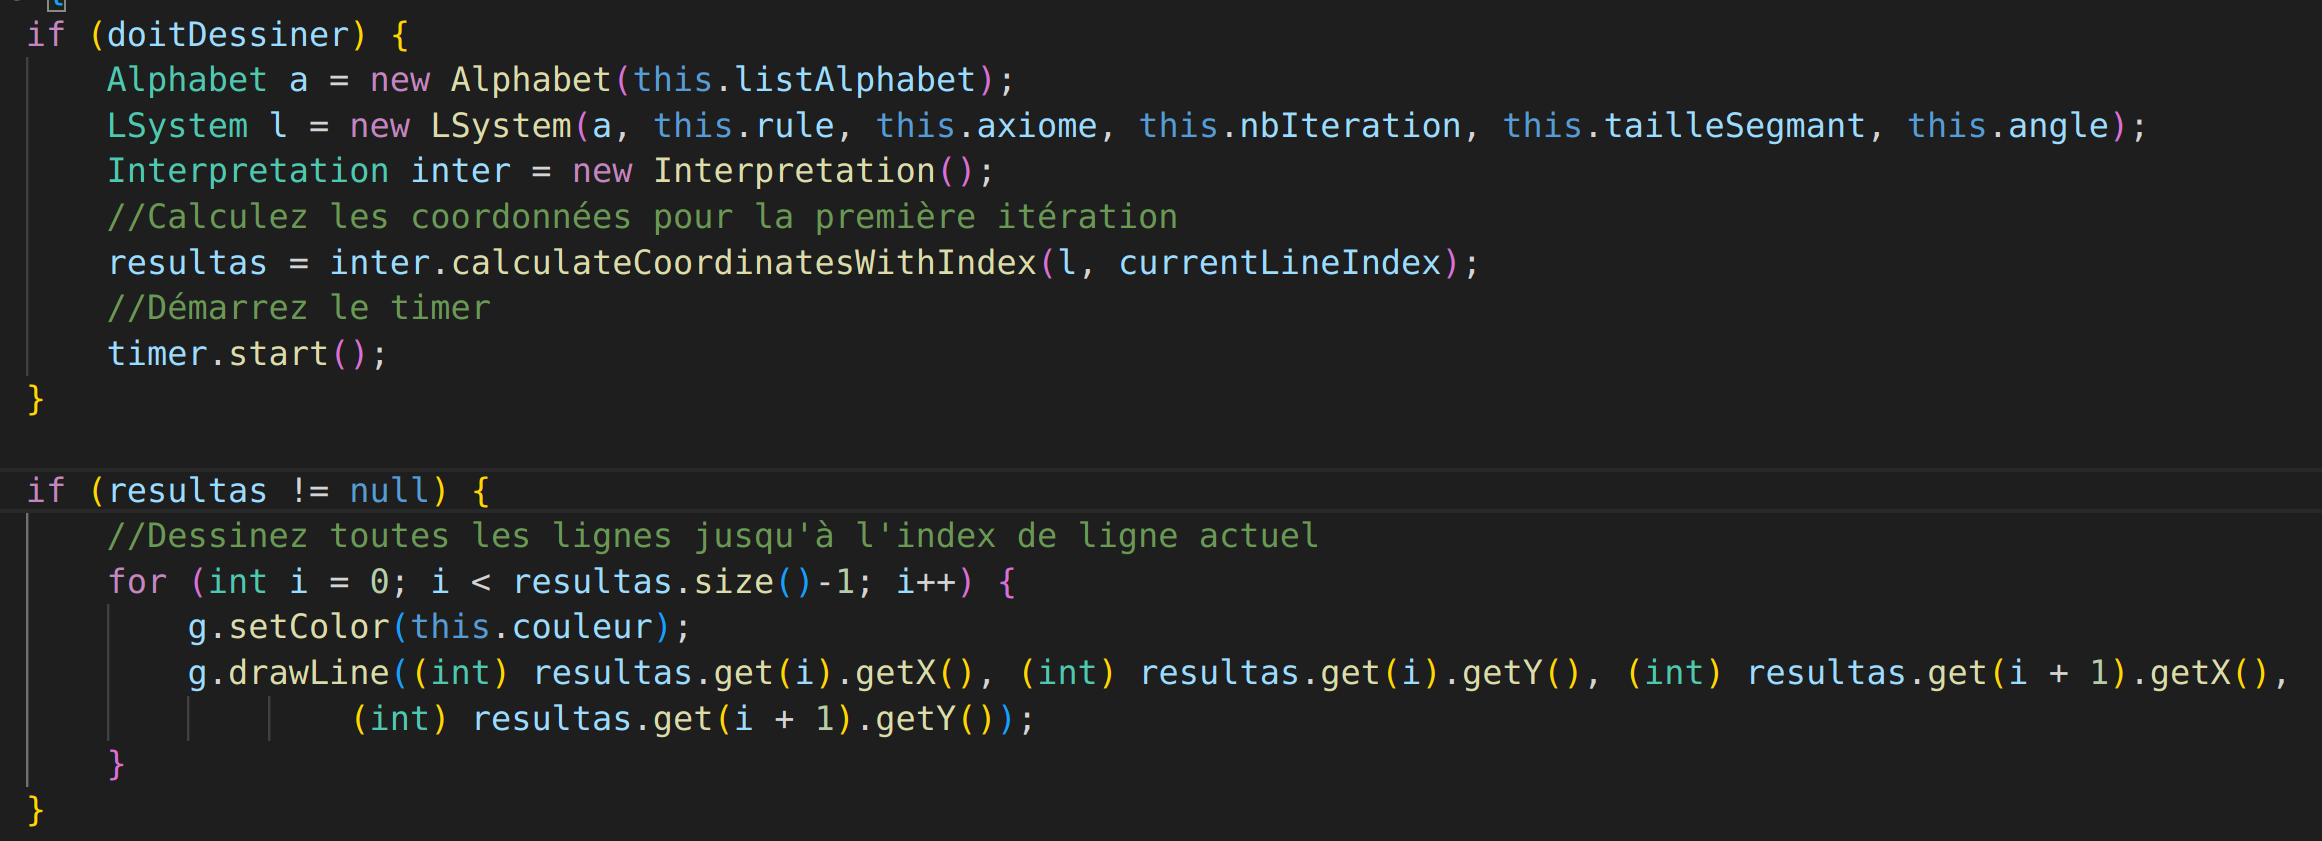
\includegraphics[width=0.5\textwidth]{images/timer4.png}
      \caption{ Timer}
      \label{fig:3D}
    \end{figure}
\end{frame}